% State of Strobe. IEEE ICCE 2027 (Las Vegas), IEEE conference template.
% Draft for co-authors. Red [TODO] marks are open; [RF] marks are for Rich Fletcher.
\documentclass[conference]{IEEEtran}
\IEEEoverridecommandlockouts
\usepackage{cite}
\usepackage{amsmath,amssymb}
\usepackage{graphicx}
\usepackage{booktabs}
\usepackage{xcolor}
\usepackage{url}
\usepackage[hidelinks]{hyperref}
\graphicspath{{figures/}}

\newcommand{\todo}[1]{\textcolor{red}{[TODO: #1]}}
\newcommand{\rf}[1]{\textcolor{blue}{[RF: #1]}}
\newcommand{\dprime}{d^{\prime}}

\begin{document}

\title{State of Strobe: What a Consumer EEG Headband Sees of Drowsiness, Eye Strain and Fatigue Under Flicker in a VR Headset}

\author{
\IEEEauthorblockN{Alexander Vicol and Steve Mann}
\IEEEauthorblockA{University of Toronto and MannLab Canada, Toronto, Canada\\
vicola.lexo@gmail.com}
}

\maketitle

\begin{abstract}
Reading an image from the eye with the steady-state visual evoked potential means minutes of 12\,Hz flicker in a headset, cell after cell, with black in between. After the first sessions the subject said the flashing seemed to make them sleepy; after a later evening of two sessions they said their eyes were irritated, their forehead ached, and they were not sleepy at all. We call the state a session leaves behind the State of Strobe and ask what a consumer headband (Muse 2 with one added occipital cup, under a Meta Quest 3S) can see of it. Twenty-three sessions over five weeks give the drowsiness answer: with the flicker line cut out of every band, theta/alpha on the occipital cup is the same while a cell flickers as while a black cell is shown seconds away (+0.001 log10, 95\% interval $-0.040$ to $+0.041$), the only drift through a session is the wet electrode settling, a fourteen-minute session with no flicker at all drifts toward the drowsy side at least as fast, and eye closure is lower under flicker, not higher. Seven sittings analysed in depth, two in one evening, three in daytime and one at half past midnight against a reference night, give the rest: the blink rate on task doubled from the first sitting of the evening to the second (7.8 to 12.0 per minute), sat at 4 to 6 in daytime and at 8.8 after midnight; blinks stop while a cell flickers and burst the moment it goes dark, most in the evening; the forehead ache is in neither the muscle nor the EEG; and the SSVEP itself faded through the second evening sitting, collapsed within two minutes after midnight on a clean electrode, and held through two morning sittings. Flicker in a headset is not sedating on these markers. What it costs is the eyes, and the same headband can tell when.
\end{abstract}

\begin{IEEEkeywords}
flicker; SSVEP; EEG; drowsiness; eye strain; blink rate; virtual reality; consumer electronics; wearable sensing; just-in-time adaptive intervention.
\end{IEEEkeywords}

\section{Introduction}

The eye-as-camera method \cite{mann2019eye} reads a picture from the SSVEP \cite{norcia2015ssvep}: a square flickers at one gaze position after another, and the response strength at each is the pixel. Our consumer version runs the stimulus in a Quest 3S browser and records with a Muse 2 headband plus one cup electrode at Oz. A session is twenty to thirty-five minutes of 12\,Hz flicker (9\,Hz for the blue plane) interleaved with black cells, in a dark headset, with the gaze held on a dot.

Two reports from the subject motivated this paper. After the early sessions, that the flashing seemed to induce drowsiness and help with sleep. After two colour sessions in one evening, that the eyes were irritated and the forehead ached, with no drowsiness. Both are about the state the strobe leaves behind, which matters for anyone who would use the method as a screening tool with a community health worker holding the laptop \cite{fletcher2010wearable, fletcher2014mental}, and for the wearable-as-window-on-state tradition that reads the body's signals in daily life and acts on them \cite{fletcher2010icalm, hernandez2013insideout, nahum2018jitai}. Flicker in the 3 to 30\,Hz band is also the stimulus that provokes photosensitive seizures \cite{fisher2005photic}, so what else it does to a person is not an idle question.

Every session we had recorded was an unplanned experiment on this: flicker and black interleaved within minutes, same electrodes, same subject. We ask the recordings three things. Is the EEG drowsier under flicker than under black seconds away, and does any drowsiness marker climb with minutes on task? What do the eyes do, blink by blink? And does the SSVEP itself hold up through a sitting? The answers come from twenty-three sessions for the drowsiness question and from seven sittings in depth for the rest, including two daytime scans, a sitting at half past midnight, a morning scan of a three-dimensional object, and one session of the same length with sound and no flicker at all. One subject throughout.

\section{Data and Methods}

\textbf{Sessions.} Twenty-three sessions between September 14 and October 17, 2026, with an Oz channel and a known delivered flicker frequency, 3 to 35 minutes of stimulation each, all at night except four. Seven are analysed in depth (Table~\ref{tab:sittings}): a reference night with no symptom report, the two colour sittings of October 10 after which the eyes and forehead were reported, a grey acuity scan at noon on October 11, a colour sitting at 10:40 on October 12, a grey portrait scan begun at 00:35 on October 17 and stopped after 48 cells, and a colour scan of a die's unfolded faces at 10:45 the same morning. One more recording is the flicker-free control the within-session contrasts lack: fourteen minutes of recorded speech played from the headset at 01:35 on October 17 with the eyes open on a dot and nothing flickering, same headband, same headset. \todo{the subject's report after the two daytime sittings}

\textbf{Markers.} Per 2\,s epoch after a 1 to 40\,Hz band-pass, with the flicker line, its harmonics and its subharmonic cut out of every band (12\,Hz and its 6\,Hz subharmonic sit inside alpha and theta and would otherwise read as drowsiness): log10 theta/alpha (4 to 7.5 over 8 to 10.5\,Hz), log10 (theta + alpha)/beta and log10 alpha power on Oz and on the ears; eye closure as the share of time with Oz alpha above three times the eyes-open baseline for a second or more. Epochs over 150\,$\mu$V or more than 20\% blink are left out. Two contrasts: \emph{acute}, each flicker epoch against the nearest black epoch within 45\,s, so time on task is matched; and \emph{drift}, the Theil-Sen slope per 10 minutes over flicker epochs and over black epochs separately, so a sedating flicker would show as the first exceeding the second.

\textbf{Blinks.} Every Muse channel is referenced at Fpz, the most blink-sensitive spot on the head, so a blink appears as one identical negative pulse of about 60\,$\mu$V on the channels far from the eyes (TP9, TP10 and the Oz cup) and only as a 3 to 16\,$\mu$V gradient on AF7 and AF8. A frontal detector counts nothing under the headset; a far-channel detector on a 0.5 to 8\,Hz band, built independently twice, agrees to the decimal. We report the blink rate on the 12\,Hz stages and in 5-minute windows, amplitude, duration, long blinks (over 400\,ms, the sleepiness sign), and a peri-event histogram around the moment a flickering cell turns black; intervals are block bootstraps over 30\,s blocks.

\textbf{Forehead.} Frontalis EMG as 20 to 45\,Hz and 65 to 120\,Hz power on AF7 and AF8 with every stimulus line and the mains cut out, its ratio to the ear and Oz channels, bursts above three times the session median, and the 60\,Hz pick-up as the contact proxy.

\textbf{The SSVEP as its own fatigue meter.} For the colour sittings, every lit cell's response (power at the flicker frequency and its harmonic over the 14 to 50\,Hz floor, the driver's own pixel value) is plotted against minutes on task next to the Oz cup's broadband noise and mains pick-up per minute, so a fading response can be told from a drying contact.

\textbf{Confounds.} Contact, whole-head movement, leakage of the stimulus line into the forehead channels, jaw muscle on the ears and the missing eyes-open baseline were each measured before any marker was read, and every October 10 finding was recomputed by two independent analyses briefed to refute it; nineteen checks completed and agreed.

\begin{table}[t]
\caption{The seven sittings analysed in depth. Blink rate is on the 12\,Hz stages; release is blinks per minute in the first second after a cell goes dark against seconds one to four; drift is log10 Oz theta/alpha per 10 minutes over flicker and over dark epochs (the midnight scan had too few dark cells for the second).}
\label{tab:sittings}
\centering
\scriptsize
\setlength{\tabcolsep}{4pt}
\begin{tabular}{lcccc}
\toprule
sitting & min & blinks/min & release & drift f / d \\
\midrule
10-07 night, ref. & 16.9 & 4.1 & 8 / 3 & $-$0.39 / $-$0.44 \\
10-10 17:57 & 20.9 & 7.8 & 27 / 10 & $-$0.15 / $-$0.04 \\
10-10 19:50 & 30.2 & 12.0 & 36 / 19 & +0.01 / $-$0.04 \\
10-11 12:05 grey & 24.9 & 4.7 & 18 / 4 & $-$0.21 / $-$0.16 \\
10-12 10:40 & 25.6 & 5.8 & 8 / 6 & +0.06 / +0.05 \\
10-17 00:35 grey & 8.1 & 8.8 & 9 / 11 & $-$0.42 / -- \\
10-17 10:45 die & 13.8 & 5.5 & 6 / 4 & $-$0.20 / $-$0.12 \\
\bottomrule
\end{tabular}
\end{table}

\section{Results}

\textbf{Drowsiness: no, on 23 sessions.} Fig.~\ref{fig:effects} pools the sessions. Acutely, with flicker on screen the EEG is not drowsier than with black on screen seconds away: Oz theta/alpha in the calibration blocks +0.009 (95\% interval $-0.053$ to $+0.071$, 9 of 19 sessions positive), in the scans +0.001 ($-0.040$ to $+0.041$); (theta + alpha)/beta and alpha power are flat as well. The one contrast below $p = 0.05$ goes the other way: on the ears, (theta + alpha)/beta is lower on the lit cell ($-0.042$, $p = 0.023$), a bright flashing field being mildly alerting, not sleep. The drift through a session is real but not from the flicker: Oz theta/alpha falls $-0.29$ log10 per 10 minutes over flicker epochs and $-0.32$ over black epochs, the same slope either way, absent on the ears, and far too large for a brain state. It is the wet cup settling, less low-frequency noise reading as less theta (Fig.~\ref{fig:courses}). Eye closure is lower under flicker than under black ($-0.021$, $p = 0.030$). The daytime sittings add nothing in either direction: the grey scan drifts like the rest ($-0.21$ and $-0.16$), the morning colour scan sits at $+0.06$ and $+0.05$, and the die scan at $-0.20$ and $-0.12$, each the same over flicker and dark. The flicker-free session settles it from the other side (Fig.~\ref{fig:flickerfree}): with speech instead of flicker, at 01:35, Oz theta/alpha was flat ($+0.01$ per 10 minutes, $-0.09$ to $+0.11$) and the ears' (theta + alpha)/beta rose $+0.16$ per 10 minutes ($+0.06$ to $+0.25$), more than the $+0.07$ it rises over flicker epochs in the 23 flicker sessions. Whatever drift there is toward the drowsy side belongs to the hour and the minutes seated, not to the strobe.

\begin{figure}[t]
\centering
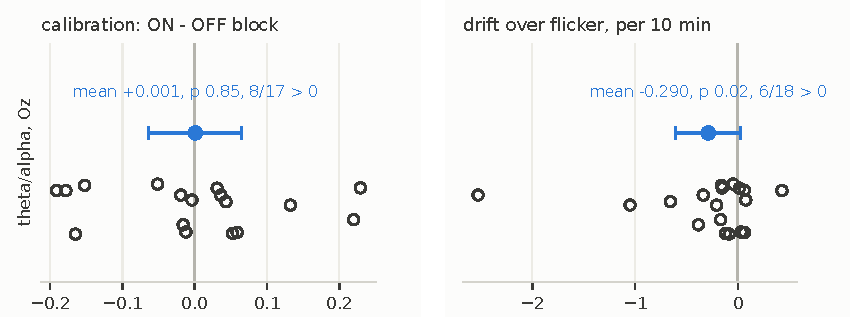
\includegraphics[width=\columnwidth]{effects_small}
\caption{Theta/alpha on the Oz cup over 21 sessions, one circle per session, the mean with its 95\% interval in blue. Left: calibration ON block minus OFF block. Right: drift per 10 minutes over the flicker epochs. Positive would be drowsier with flicker.}
\label{fig:effects}
\end{figure}

\begin{figure}[t]
\centering
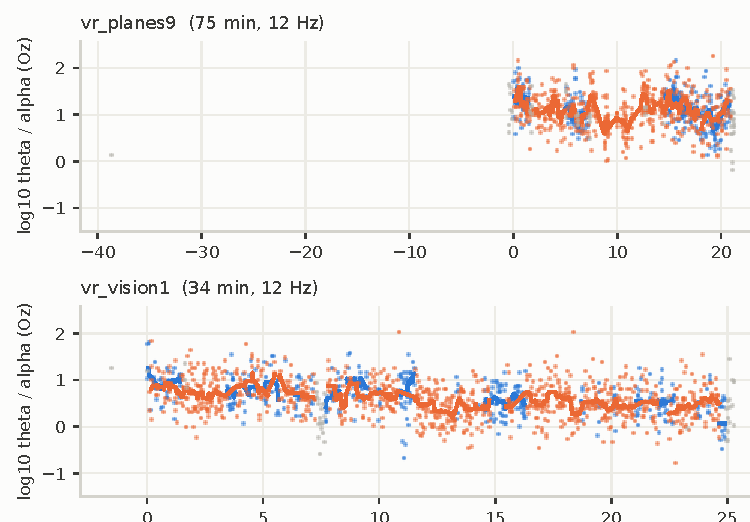
\includegraphics[width=0.8\columnwidth]{time_courses_two}
\caption{Theta/alpha on Oz through two long sessions, flicker epochs blue, black epochs orange, 30\,s running medians. Any slope is the same for both: the electrode, not the stimulus.}
\label{fig:courses}
\end{figure}

\begin{figure}[t]
\centering
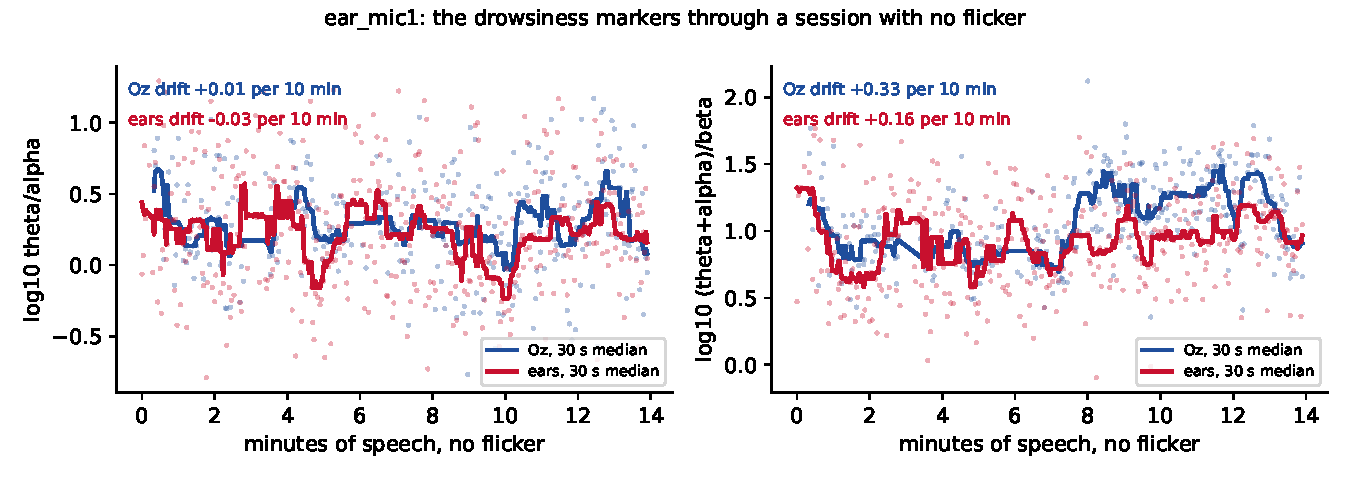
\includegraphics[width=\columnwidth]{flicker_free}
\caption{The flicker-free control: theta/alpha (left) and (theta + alpha)/beta (right) on Oz and on the ears through fourteen minutes of recorded speech from the headset at 01:35, nothing flickering, 30\,s medians. The drowsy-side rise on the ears is as large as any flicker session's.}
\label{fig:flickerfree}
\end{figure}

\textbf{The eyes: strained by the second sitting of an evening.} Fig.~\ref{fig:blinks} and Table~\ref{tab:sittings}. On October 10 the blink rate on task was 7.8 per minute in the first sitting and 12.0 in the second, against 4.1 on the reference night, and the second sitting ran at twice the first at matched minutes (+6.1 per minute, 95\% interval +4.3 to +7.9, permutation $p < 0.001$) from its first five minutes (14.0 against 4.5), with the rate flat within each sitting. Blink amplitude and duration were unchanged, so the eye blinked more, not differently: the signature of a drying, irritated cornea \cite{stern1994blink, sheedy2003cvs}. The two daytime sittings, each the first of its day, sat at 4.7 and 5.8 per minute, with the reference night and with each other, and both rose by about half from their first half to their second (3.7 to 5.7 and 3.7 to 5.8), a within-sitting climb that neither evening sitting showed. The evening doubling is therefore not what a sitting does to the eyes by itself. It is what a second sitting does after a first one and the hour between. The two October 17 sittings fall where the hour predicts: the grey scan begun at 00:35, the first sitting of its night, ran at 8.8 per minute, with the first evening sitting of October 10; the die scan at 10:45, rested, at 5.5, with the daytime ones.

\begin{figure}[t]
\centering
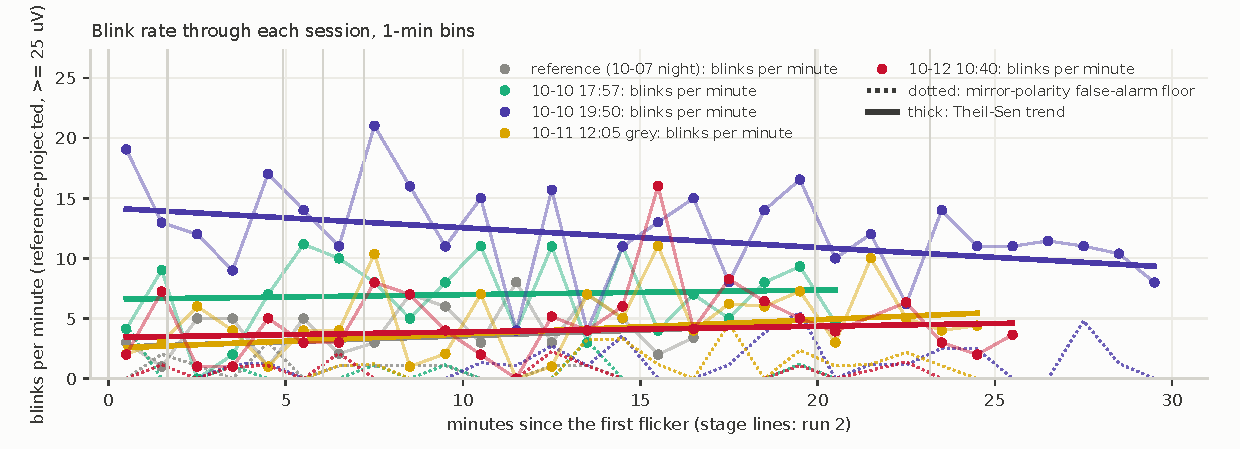
\includegraphics[width=0.92\columnwidth]{blink_rate}
\caption{Blink rate through the five sittings in 1-minute bins, with Theil-Sen trends. The second sitting of October 10 (violet) runs at twice the first (green) from its first minutes; the two daytime sittings (yellow, red) sit with the reference night (grey).}
\label{fig:blinks}
\end{figure}

\textbf{Blinks held back under flicker, released on black.} While a 12\,Hz cell flickered the subject nearly stopped blinking (2 to 5 per minute) and let a burst go the moment it went dark: 27 and 36 blinks per minute in the first second after the cell turned black on the two evening sittings, against 10 and 19 in the following three seconds (Fig.~\ref{fig:release}). The reference night showed the same shape at a lower level (8 against 3), the daytime grey scan a clear one (18 against 4), and the morning colour scan almost none (8 against 6). The right panel of Fig.~\ref{fig:release} gives the same thing as rates on lit cells, black cells and the rest breaks, where the rate reaches 20 to 35 per minute. Suppress-then-release is eyes held open on a bright target, which is how a cornea dries, and it was strongest where the blink rate was highest. No long blinks appeared at any point (0 to 1\% over 400\,ms), the sleepiness sign.

\begin{figure}[t]
\centering
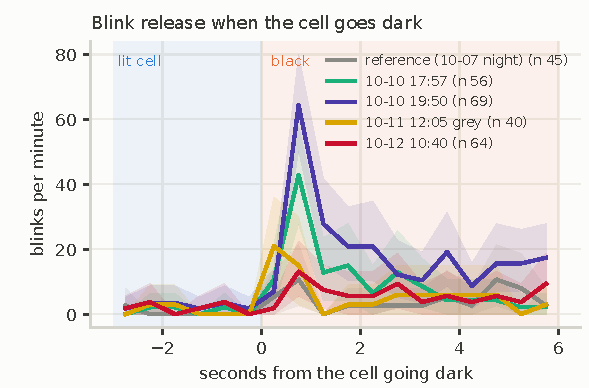
\includegraphics[width=0.49\columnwidth]{blink_release}\hfill
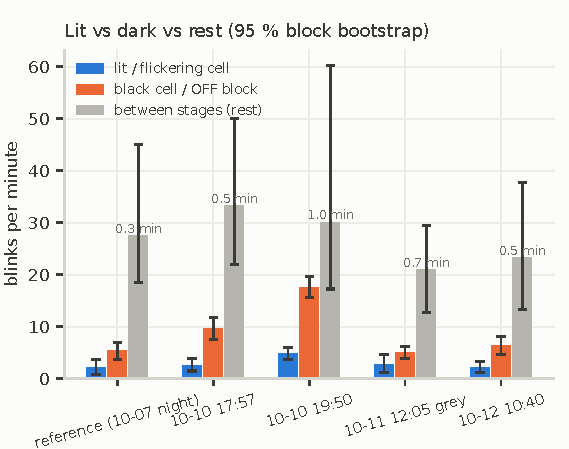
\includegraphics[width=0.43\columnwidth]{lit_dark_rest}
\caption{Left: blinks per minute in half-second bins around the moment a flickering cell turns black, per sitting, 95\% block-bootstrap bands. Right: the blink rate on lit cells, on black cells, and in the rest breaks between stages.}
\label{fig:release}
\end{figure}

\textbf{The forehead: not in the muscle, not in the EEG.} Frontalis power sat at 1.5 to 2.3\,$\mu$V rms in all three October sittings analysed for it, 10 to 100 times below a sustained contraction, with the sitting before the report at the lowest level and falling (Fig.~\ref{fig:forehead}). One episode, the left forehead electrode's broadband power tripling for the last three minutes of the first sitting, is undecidable between muscle and a shifting pad. Frontal theta did not rise with the flicker ($-5$ to $-13$\%), did not climb within any sitting, and matched the reference night. A headache has no EEG signature and the forehead electrodes show nothing that would accompany one; the headset's facial interface, which the EEG cannot see, is the likelier cause. An earlier reading of rising ear alpha in the second sitting was the right ear electrode coming loose at minute 11 and is retracted.

\begin{figure}[t]
\centering
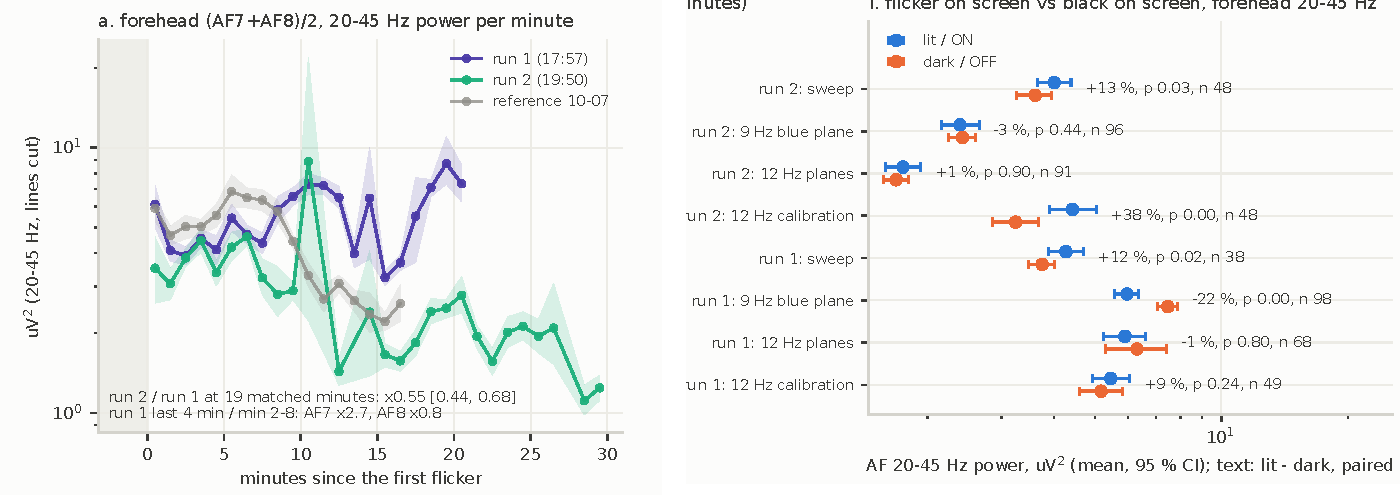
\includegraphics[width=\columnwidth]{forehead_small}
\caption{Forehead muscle through the two sittings of October 10 and the reference night. Left: 20 to 45\,Hz power per minute on AF7 and AF8 with the stimulus lines and mains cut. Right: the same band while a cell is lit against while it is black, per stage. Nothing rises toward the report.}
\label{fig:forehead}
\end{figure}

\textbf{The SSVEP as a fatigue meter.} Fig.~\ref{fig:fatigue}. The two evening sittings began in the same state (colour calibrations red +5.0, green +4.3, blue +5.5 against +5.8, +3.9, +5.0). In the second, blue's response on a clean Oz contact fell from 0.34 to 0.19 between its passes, and red and green, scanned at minutes 20 to 30, read at half the first sitting's level while the cup's own noise rose from minute 20, so for those two the electrode is the simpler explanation. The morning sitting two days later tells the other side: red held at 0.53 to 0.73 through its scan, green at 0.24 to 0.32 and blue at 0.29 to 0.41, no fading, even though the cup had calibrated at its weakest ($\dprime$ 1.8 against 5.6). October 17 gave both sides within ten hours. At 00:35, after a strong calibration ($\dprime$ 3.3 on the cup), the 12\,Hz response fell from calibration strength to the OFF-block level within two minutes of scanning and never followed the grey shown (first two minutes 3.1 times the noise floor, after that 1.2, against 7.7 in the calibration ON blocks and 1.0 OFF), with the cup clean throughout at 35 to 40\,$\mu$V and never at the rail; the sitting was stopped at 48 cells. At 10:45, rested, the die's 54 cells came back 51 right, red at 0.73 to 0.86 and 0.32 to 0.42 by quarter, green 0.26 to 0.30 and blue 0.42 to 0.52, with no trend and the cleanest cup of all (26 to 10\,$\mu$V, mains under 6\,$\mu$V). Fig.~\ref{fig:summary} puts the seven sittings side by side.

\begin{figure}[t]
\centering
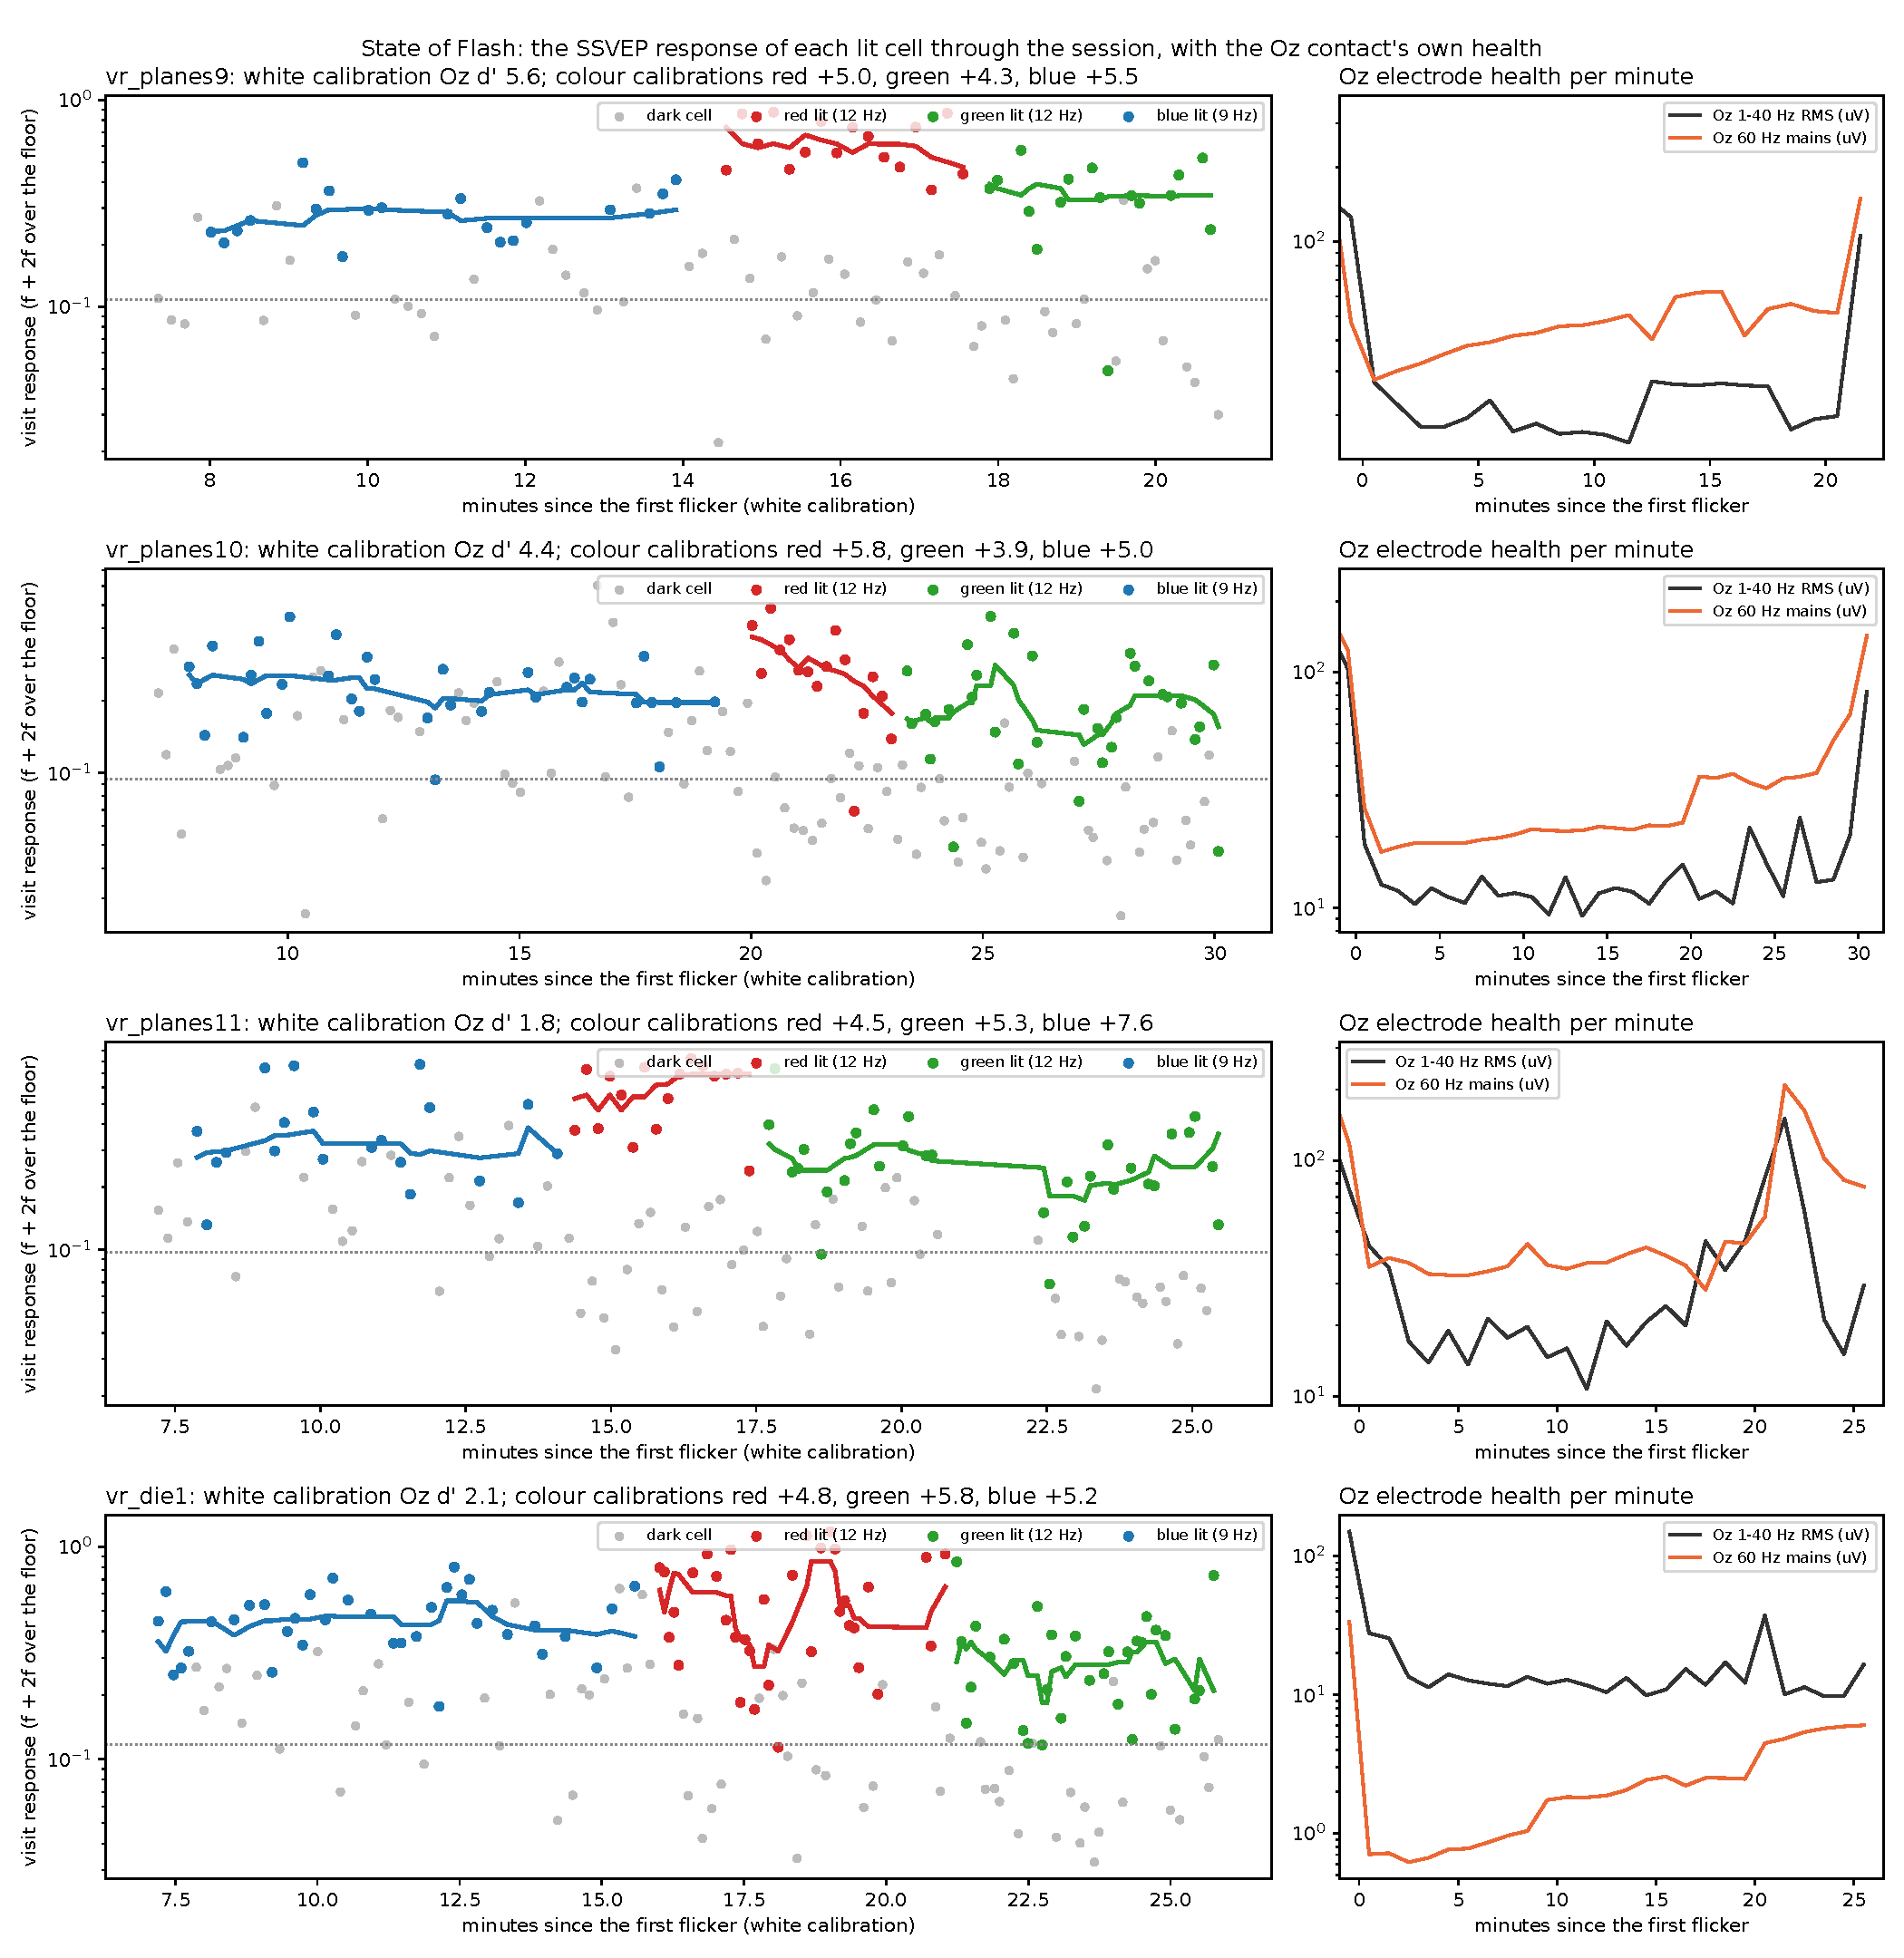
\includegraphics[width=\columnwidth]{ssvep_fatigue_four}
\caption{Every lit cell's SSVEP against minutes on task for the four colour sittings, top to bottom October 10 at 17:57, October 10 at 19:50, October 12 and the die on October 17, each beside the Oz cup's noise and mains pick-up per minute. The second evening sitting fades; the two morning sittings hold.}
\label{fig:fatigue}
\end{figure}

\begin{figure*}[t]
\centering
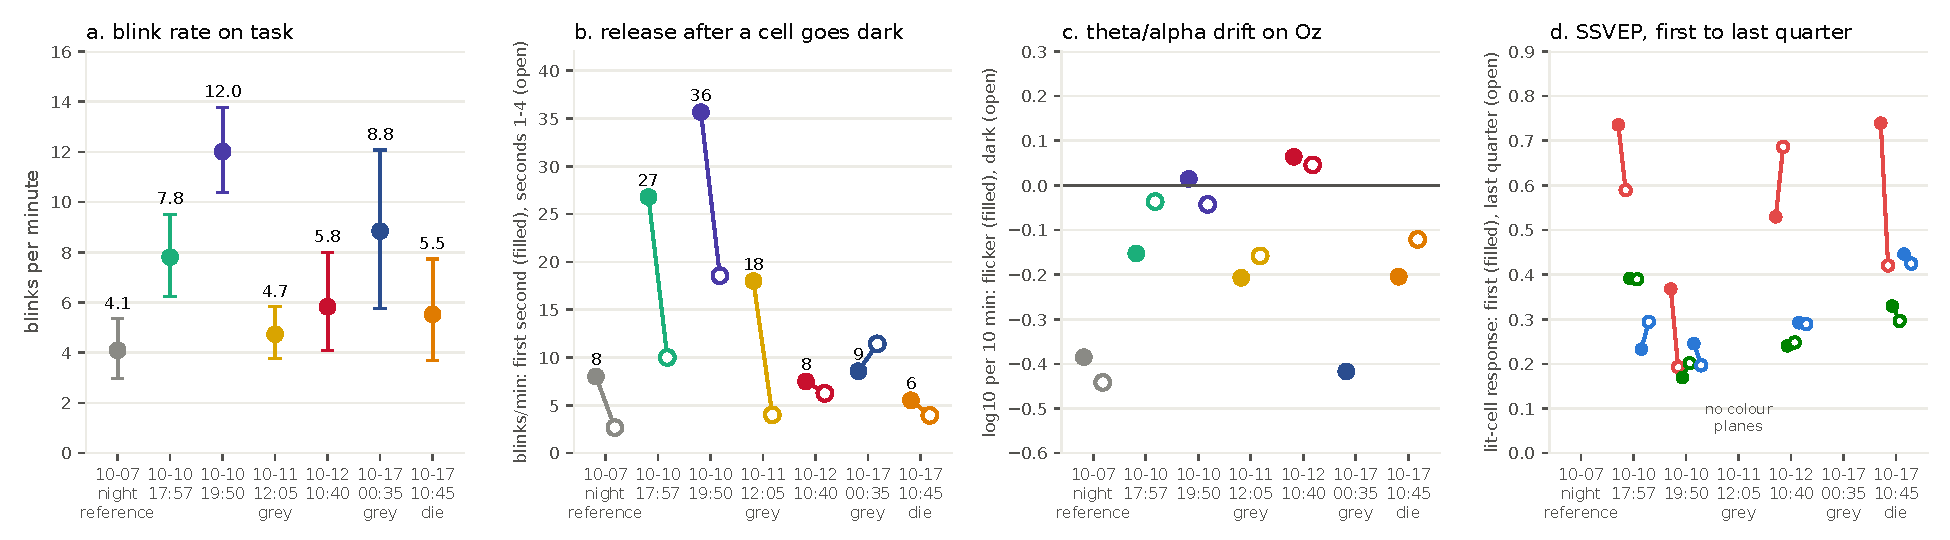
\includegraphics[width=0.68\textwidth]{summary}
\caption{The seven sittings at a glance. a: blink rate on task. b: blinks per minute in the first second after a cell goes dark (filled) against seconds one to four (open). c: Oz theta/alpha drift per 10 minutes over flicker (filled) and dark (open) epochs. d: the lit-cell SSVEP in the first (filled) and last (open) quarter of each plane's scan, red, green and blue.}
\label{fig:summary}
\end{figure*}

\section{What It Means}

\textbf{For the subject.} Flicker at 12\,Hz in a headset, in sittings of twenty to thirty-five minutes, did not make this subject drowsy on any marker the headband can measure: not acutely, not over a sitting, not on twenty-one sessions. What it did was dry the eyes, and the headband saw it two ways. The report of sleepiness after the early sessions is not contradicted by this; it is simply not in the EEG, and several of those sessions were recorded around two in the morning, when the hour explains more than the screen. The published after-effect of alpha-band flicker is a drop in alpha power, not a slide toward theta \cite{herrmann2001flicker}, consistent with what we see and not a sleep-onset signature.

\textbf{For the camera.} One sitting per evening: the second began with the eyes blinking twice as fast and read 20 of 32 colour cells where the first read 24. A pass is only worth averaging in when the electrodes held through it, so a loose-channel guard belongs in the decoder. And rest breaks are where the eyes recover, at five to ten times the rate on task, so a break every forty cells is part of the measurement.

\textbf{For a screener.} The same recording that gives the picture gives the eye-strain reading, live, from the far channels, with no extra sensor. A ``rest your eyes'' prompt on the page when the release pattern sharpens or the rate crosses a threshold is the simplest just-in-time intervention \cite{nahum2018jitai} and the first the system should carry, in the tradition of sensor-plus-app systems that read a state and answer it \cite{fletcher2011cbt, boyer2012iheal, leonard2018homeless}. Screen exposure itself has been measured from a wearable before \cite{fletcher2016screentime}; what is new here is the eye's own response to it.

\textbf{Limits.} One subject, one headband, one headset. Drowsiness after a session, rather than during it, is invisible to a within-session contrast. There is no sleepiness rating and no reaction-time test, and the one flicker-free control is a single night session with sound in place of flicker rather than silence, so the eye-strain result is a between-sitting difference with the time of evening confounded. The forehead electrodes sit at the noise floor under the headset and the blink detector is new. Flicker in this band must never be used with anyone with a history of photosensitive epilepsy \cite{fisher2005photic}.

\section{A Study That Could Answer It}

The stimulus page already does everything needed; what is missing is the design and two questions to the subject. Five-minute blocks, counterbalanced and at matched luminance: full-field 12\,Hz flicker, static grey at the same mean luminance, and black with the dot; a sleepiness rating before and after every block \cite{akerstedt1990kss} and a two-minute reaction-time test after each \cite{dinges1985pvt}, both on the page; the Oz cup given five minutes to settle first; a block at the subject's own alpha frequency and one at 40\,Hz; daytime as well as night; more than one person. Three sessions of under an hour would turn ``it seems to make me sleepy'' into a number with an interval around it.

\section{Conclusion}

On every drowsiness marker a consumer headband can measure under a VR headset, 12\,Hz flicker interleaved with black is not sedating, acutely or over a sitting, on twenty-three sessions of one subject, and a session of the same length with no flicker drifts toward the drowsy side at least as fast. The state the strobe leaves behind is in the eyes: a blink rate that doubles on the second sitting of an evening and blinks held back under the flicker and released on black, with the blink itself unchanged and no sign of sleep. The forehead ache is not in the forehead's muscle or EEG. The SSVEP fades through a second evening sitting, collapses within minutes after midnight on a clean electrode, and holds through fresh morning sittings. For the camera that means one sitting per evening, rest breaks as part of the measurement and a contact guard; for a screener it means the eye-strain reading comes free with the picture, and the prompt to rest the eyes can come from the same headband.

\section*{Acknowledgements}
\todo{MannLab Canada; Interaxon. Confirm wording.}

\bibliographystyle{IEEEtran}
\bibliography{refs}

\end{document}
